\chapter{Une interface de recherche adaptée}
Une fois que les données RDF produites sont chargées dans une base de graphes et rendues exploitables, il convient de les doter d'une interface de recherche pour ses futurs utilisateurs. Proposer uniquement l'éditeur de requêtes SPARQL brut, comme l'offre n'importe quel SPARQL end point, ne suffit pas : la grande majorité des utilisateurs finaux de données historiques ou archivistiques ne connaissent bien évidemment ni SPARQL ni l'ontologie de référence. En outre, exploiter véritablement un graphe, qui relie des entités appartenant à un nombre significatif de classes distinctes, par un nombre significatif de relations différentes, ne peut pas se faire par des biais classiques tel qu'un formulaire de recherche avancée. Il est nécessaire de trouver une solution permettant à l'utilisateur d'explorer ce graphe à sa guise. Dans le temps limité qui nous était imparti, nous avons choisi d'utiliser l'outil Sparnatural.
\begin{figure}[h]
    \centering
    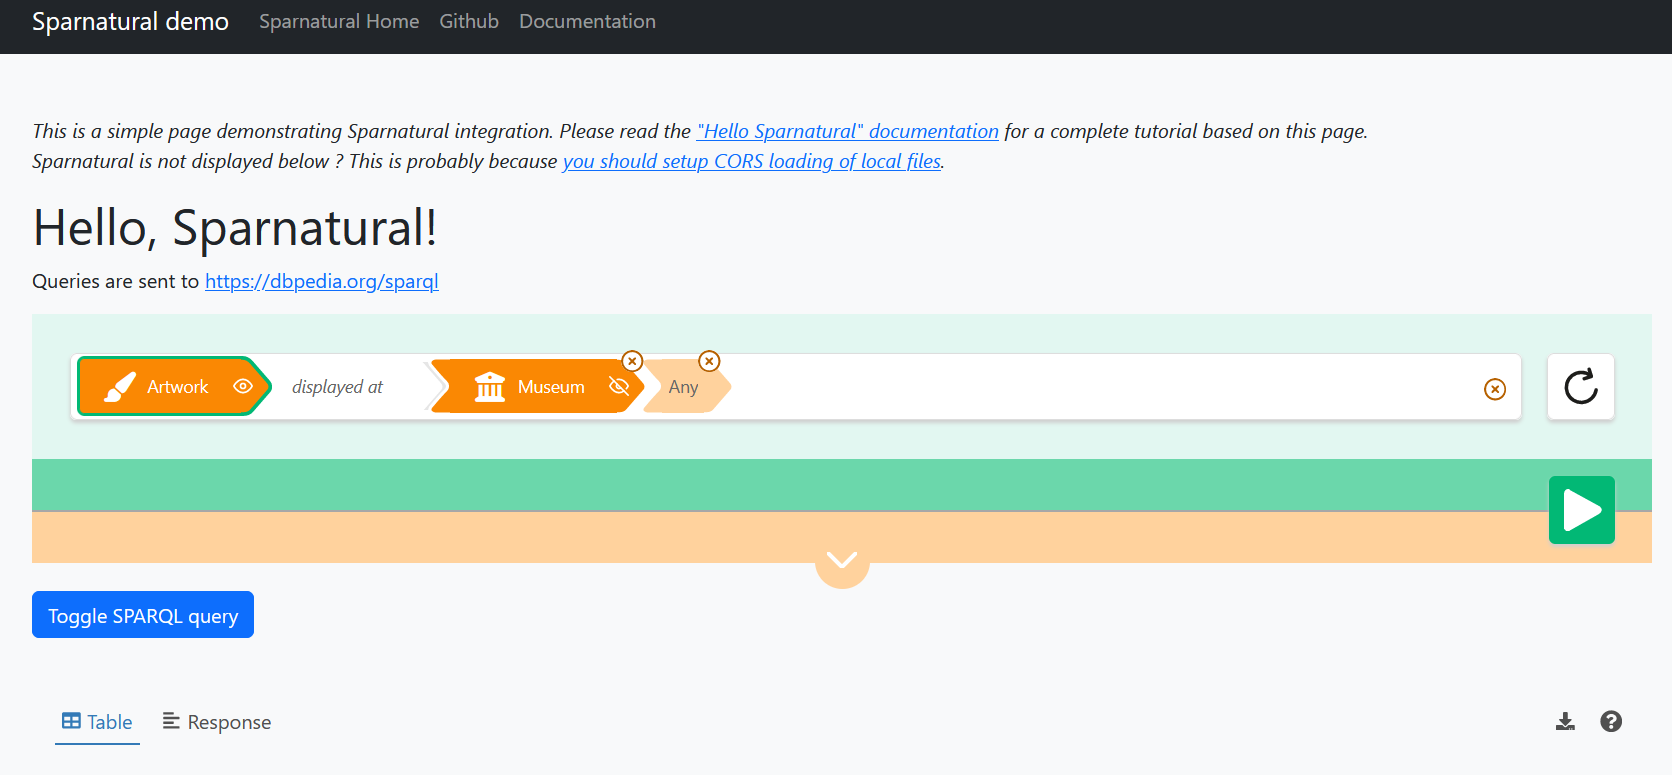
\includegraphics[width=1\linewidth]{images/hello sparnatural.png}
    \caption{L'exemple de la configuration classique de l'outil Sparnatural. Ici la requête interroge la base de données DB Pedia sur les oeuvres d'arts qui sont affichées dans n'importe quel musée.}
    \label{fig:hello-sparnatural}
\end{figure}
\section{La solution Sparnatural}
\subsection{Une interface sur mesure}
Sparnatural est un éditeur visuel open source et gratuit de requêtes SPARQL. Développé en JavaScript par 
la société Sparna, il permet à l'utilisateur de construire visuellement un questionnaire qui sera automatiquement traduit en requête SPARQL par l'outil. L'outil a d'abord été développé en 2018 par Sparna pour pouvoir doter le portail OpenArchaeo d'une interface web de recherche. Ses fonctionnalités, son design et sa documentation ont ensuite été fortement améliorés en 2021-2022, dans le cadre d'un projet associant la BnF, le ministère de la Culture et les Archives nationales (via le Lab qui a porté ce projet), qui a également permis à la BnF \footnote{Voici le lien du démonstrateur de la BNF : \href{https://data.bnf.fr/sparnatural/}{https://data.bnf.fr/sparnatural/}}et aux Archives nationales, en juin 2022, de mettre en ligne deux démonstrateurs. Le démonstrateur des Archives nationales a été réalisé par le Lab en collaboration avec Sparna et propose aujourd'hui deux interfaces de recherche. Il va très probablement évoluer en 2024, en même temps que l'outil, dans le cadre d'une troisième phase. Voyant les bons résultats ainsi obtenus pour des données RDF/RiC-O, l'équipe projet du portail FranceArchives a décidé de sémantiser les métadonnées du portail conformément à RiC-O 0.2 et de les rendre interrogeables via une interface utilisant également Sparnatural, publiée en septembre 2023. Compte tenu de ces précédentes expériences sur des projets d'envergure et des qualités de l'outil, il était logique d'envisager de l'utiliser également pour le futur portail ORESM. Nous avons pu avoir accès à une documentation avant sa publication. Cette documentation est très bien renseignée, une partie de celle-ci explique pas à pas la configuration d'une interface basique, et une autre montre l'ensemble des possibilités en configurant l'outil à l'aide d'une ontologie OWL. Il est à noter que les résultats des requêtes peuvent s'exporter au format CSV. Pour la réalisation d'une première interface de recherche, pour les données RDF que nous avions produites, nous avons utilisé la version 8.5 de Sparnatural, publiée en juillet dernier, et nous sommes partis de la configuration réalisée par Florence Clavaud pour la preuve de concept initiale.
\par
L'outil permet d'envoyer des requêtes à un Sparql Endpoint et d'afficher les résultats comme dans n'importe quel éditeur de requête SPARQL. La différence réside dans l'élaboration d'une interface qui représente les triplets interrogés d'une manière visuelle. On clique sur des boutons pour naviguer entre les possibilités définies par la configuration de l'interface. De cette manière l'utilisateur n'est pas obligé de connaître le modèle de données, mais il doit tout de même élaborer sa recherche d'une manière conceptuelle : quelles sont les entités qu'il recherche ? Quelles sont les caractéristiques ou les relations de ces entités sur lesquelles il veut effectuer sa recherche ? La conception d'une requête reste à appréhender, mais on a éliminé le problème de la connaissance de l'ontologie et du langage SPARQL. 
\par
Pourtant Sparnatural est agnostique, c'est à dire qu'il est utilisable pour n'importe quel jeu de données RDF conforme à n'importe quelle ontologie. C'est lors de sa configuration, qui peut notamment se faire via un fichier OWL\footnote{Le fichier OWL est le type de fichier utilisé pour construire une ontologie.}, qu'on définit quelles entités et quelles relations l'utilisateur final va pouvoir employer dans la construction de sa requête. Il s'agit finalement de \textit{"spécifier un modèle ontologique pour la recherche et ses correspondances avec les classes et propriétés de l’ontologie métier"}.\footnote{Citation tirée de la documentation du projet de démonstrateur des AN : \href{https://sparna-git.github.io/sparnatural-demonstrateur-an/presentation-fr.html\#design}{https://sparna-git.github.io/sparnatural-demonstrateur-an/presentation-fr.html\#design}}


\subsection{Modélisation de l'interface}
Nous avons donc choisi cette méthode de configuration par une ontologie. Il y a d'abord eu un travail de modélisation à faire. Puisque l'idée initiale de la preuve de concept était de traiter absolument toutes les données contenues dans les fichiers Excel de dépouillements, alors il fallait pouvoir toutes les interroger pour permettre une relecture. Nous avons réalisé une modélisation avant de nous lancer dans la configuration, des critères de requête nécessaires pour interroger l'ensemble de nos données (voir le schéma de modélisation ci-dessous). Dans cette modélisation, on voit que la majorité des types d'information que nous avons sont liés à la pièce d'archives. Tout passe par la ressource archivistique qui reste la composante essentielle de la majorité de nos triplets. Avec cette configuration plus besoin de différencier, comme dans le modèle RiC-O, le RecordResource et l'Instantiation, c'est une notion qui est utile en terme de gestion de données mais ne servira à rien pour le chercheur utilisateur. Certains choix ont été faits aussi concernant la question du sceau. Nous avons décidé de créer un critère particulier pour les relations entre une ressource archivistique et son sceau. Utiliser directement, comme c'était exprimé dans les tableaux de dépouillements et l'ontologie ORESM, un critère sur les caractéristiques physiques aurait rendu la recherche malaisée. Nous avons beaucoup de granularités dans nos données, et dans un cas comme le nôtre il ne faut pas surcharger l'interface d'éléments au risque de perdre et décourager l'utilisateur mais il ne faut pas non plus trop limiter les possibilités de recherche pour les utilisateurs déterminés. Il faut chercher à \textit{" atteindre par ce biais un compromis raisonnable entre la complexité du modèle métier et la nécessité de produire une interface compréhensible et performante pour les utilisateurs"}\footnote{Citation tirée de la documentation du projet du démonstrateur des AN : \href{https://sparna-git.github.io/sparnatural-demonstrateur-an/presentation-fr.html\#design}{https://sparna-git.github.io/sparnatural-demonstrateur-an/presentation-fr.html\#design}}

\begin{figure}[h]
    \centering
    \includegraphics[width=1.1\linewidth]{images/sparnatural shéma.PNG}
    \caption{Modélisation du système de requête dans notre interface Sparnatural}
    \label{fig:shéma_sparnatural}
\end{figure}

\section{La configuration ORESM}
\subsection{Édition sur Protégé}
Puisque le fichier de configuration se base sur le langage OWL, il est possible de l'éditer avec le logiciel Protégé. La logique hiérarchique des classes importe peu, on les distingue en deux types, les classes représentant des types d'entités RDF, et associées à un ou plusieurs URI, et les classes qu'on appelle littérales qui permettent d'accéder aux Datatypes properties. La configuration de l'interface pour les classes nous a paru assez simple puisque nous disposions d'une bonne documentation, que nous connaissions nos données, l'ontologie ORESM et avions défini notre modèle de requêtes. On peut donner des attributs aux différentes classes, ils permettent d'afficher davantage d'informations à l'utilisateur. L'attribut \textit{tooltip} permet d'afficher un message de description lorsque le curseur est sur l'objet concerné. Il est également recommandé d'utiliser des icônes pour améliorer l'expérience utilisateur, pour ce faire il faut indiquer pour la valeur de l'attribut \textit{fontawesome icon code} le code associé à cette icône sur le site \href{https://fontawesome.com/}{Font Awesome}. On peut aussi spécifier l'ordre d'apparition des classes qui seront les premiers points d'entrée dans le graphe, avec l'attribut \textit{order}.
\begin{figure}[h]
    \centering
    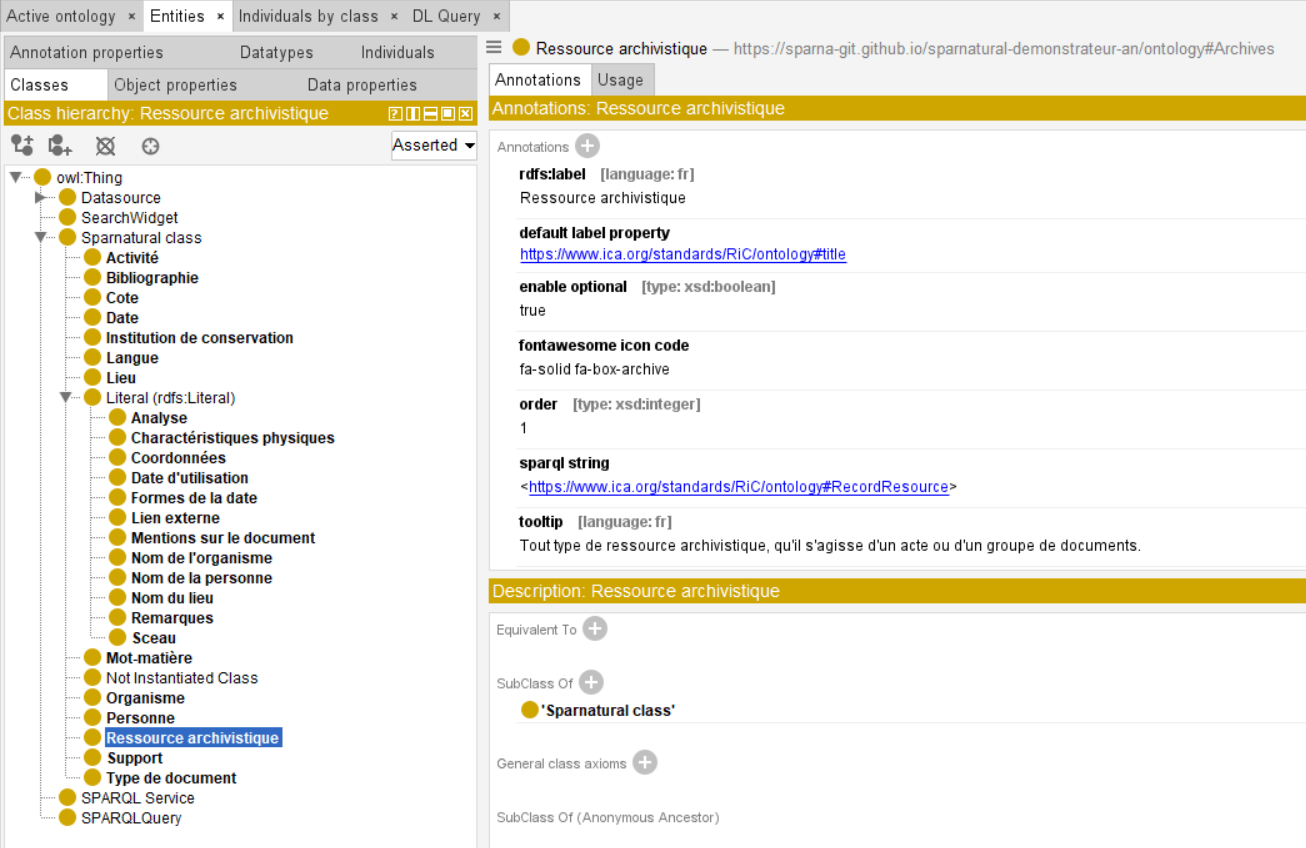
\includegraphics[width=0.9\linewidth]{images/classes sparnatural.png}
    \caption{Capture d'écran des classes créées pour la configuration de l'interface Sparnatural avec les attributs des Ressources Archivistiques.}
    \label{fig:classes-sparnatural}
\end{figure}

Pour ce qui est des relations, plusieurs catégories sont mises à disposition. Quand il s'agit d'une relation ayant pour cible une classe d'entités, un système de liste ou d'auto-complétion permet de viser une entité précise en parcourant les données avant même d'avoir exécuté la requête\footnote{Ces dispositifs permettent en général d'interroger la datatype property rdfs:label d'une instance de classe.}. Une liste est plus efficace pour un nombre restreint d'éléments, c'est l'inverse pour l'auto-complétion. Les autres liens, ceux visant des valeurs littérales peuvent être de plusieurs catégories ; en fonction de ces catégories l'interface proposera différentes manières de filtrer la valeur. On peut disposer d'une simple zone de saisie, d'un choix booléen, d'une carte pour sélectionner des coordonnées géographiques ou même d'un calendrier pour choisir un intervalle de date. Évidemment ces options servent à appliquer un filtre sur les données mais pour chacune d'entre elles on peut également décider d'accepter toutes les valeurs. Pour ce qui est de l'interprétation en SPARQL il faut remplir le champ \textbf{sparql string}\footnote{Voir ci dessous l'exemple de valeur qu'il peut prendre.}. 
\par
Prenons l'exemple qui concerne le lien \textbf{est conservé actuellement par}. On spécifie que cette relation part (on dit qu'elle a pour domaine)  de la "Ressource Archivistique" et cible (on dit qu'elle a pour portée) une "Institution de conservation", respectivement un rico:RecordResource et un rico:CorporateBody. Sparnatural utilise pour générer ses requêtes les possibilités offertes par SPARQL pour parcourir un graphe de manière concise. On indique simplement la relation en utilisant la syntaxe proposé par le W3C\footnote{\href{https://www.w3.org/TR/sparql11-query/\#propertypaths}{Lien des spécifications W3C concernant la syntaxe des Property Path}}. Sparnatural met également à disposition un éditeur de requête SPARQL. On peut donc voir l'équivalent en SPARQL des requêtes construites avec l'éditeur visuel. Les personnes connaissant le langage préféreront sans doute y saisir directement leurs requêtes puisque cela permettra davantage de possibilités mais il n'y a aucune assistance à la saisie (par exemple pas d'auto-complétion).

\begin{figure}[h]
    \centering
    \includegraphics[width=1\linewidth]{images/sparnatural est conservé.png}
    \caption{Valeur du champ sparql string qui contient une expression SPARQL utilisée pour la relation \textbf{est conservé actuellement par}.}
    \label{fig:lien-sparnatural-conserve}
\end{figure}
\begin{figure}[h]
    \centering
    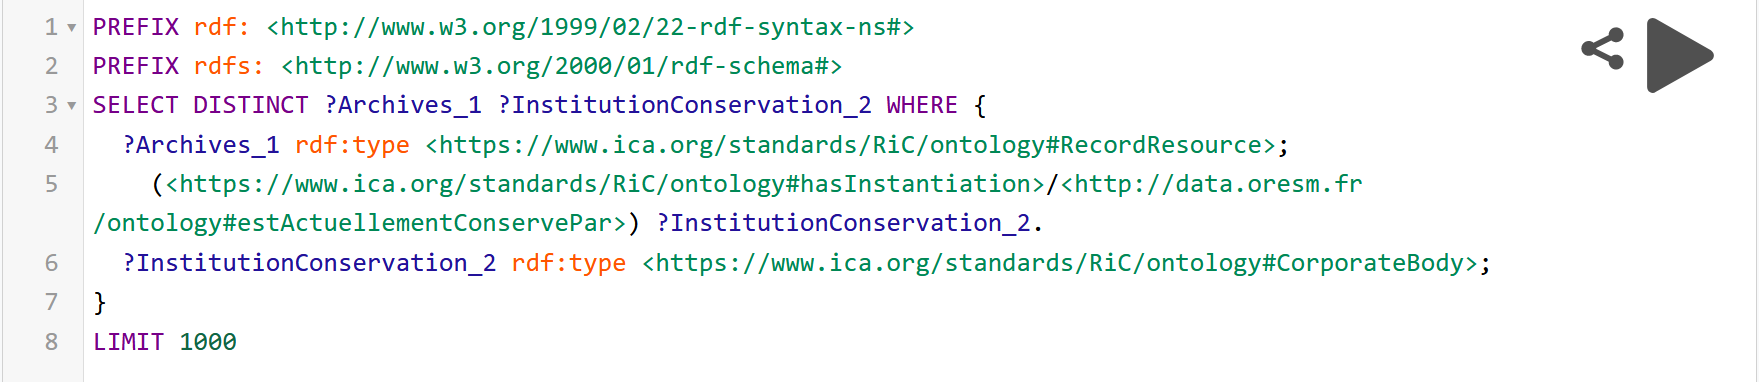
\includegraphics[width=1\linewidth]{images/equivalent sparql.png}
    \caption{Équivalent de cette relation dans l'éditeur de requête SPARQL.}
    \label{fig:lien-sparql-conserve}
\end{figure}

\subsection{Présentation de l'interface}
Finalement nous avons décidé de configurer deux interfaces, la première pour la recherche avancée, qui se base sur le modèle présenté plus tôt, et une autre de recherche simple. Celle-ci veut simuler une recherche plein texte avec l'outil Sparnatural ; ce n'est absolument pas une configuration définitive (tout comme celle avancée d'ailleurs). La recherche simple est présente pour voir si il était possible de faire ce type de recherche sur les données. La valeur écrite dans la zone de saisie est recherchée dans l'ensemble des rdfs:label de nos entités. C'est donc techniquement faisable mais il faudra revoir l'interface. Les réponses sont rapides, toujours en dessous de 0,5 seconde, ce qui était la principale inquiétude de cette recherche plein texte.\footnote{Pour ce type de recherche l'interface ORESM devrait pouvoir bénéficier en 2024 d'une évolution de Sparnatural qui irait en ce sens.} Voici quelques captures d'écran de l'interface utilisée.

\begin{figure}[!h]
    \centering
    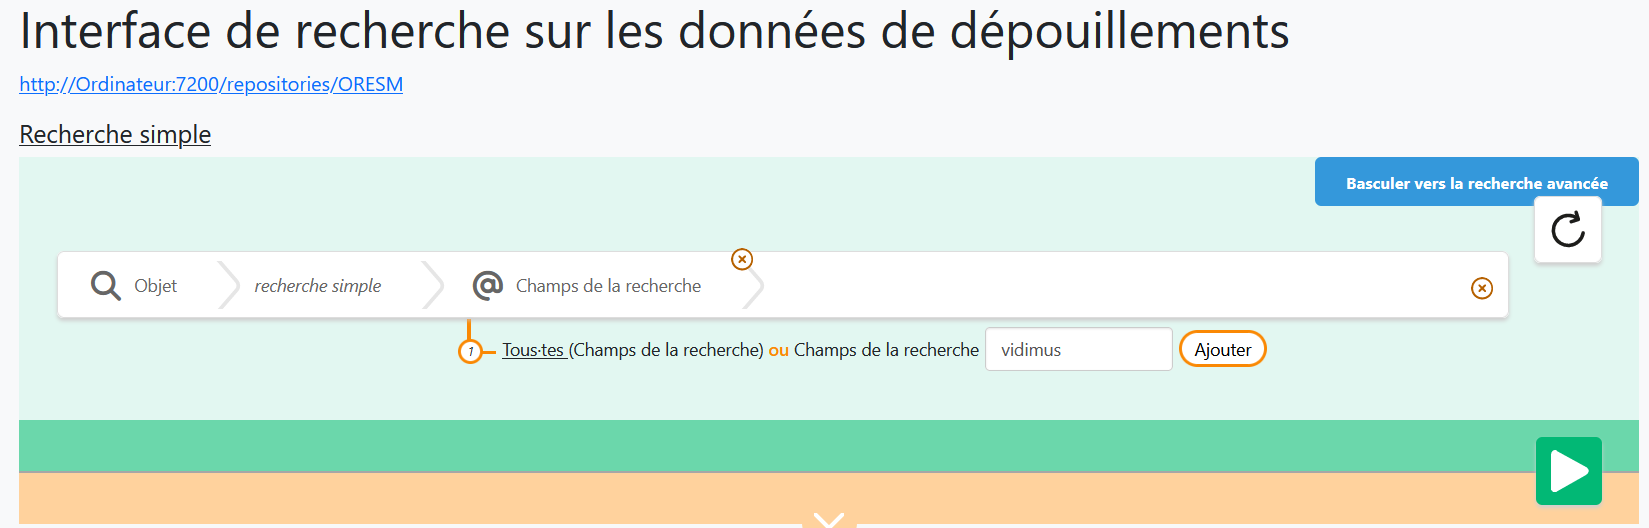
\includegraphics[width=1.1\linewidth]{images/recherche-simple.png}
    \caption{Interface de la recherche simple. On ne peut sélectionner qu'un unique élément.}
    \label{fig:recherche-simple}
\end{figure}
\begin{figure}[!ht]
    \centering
    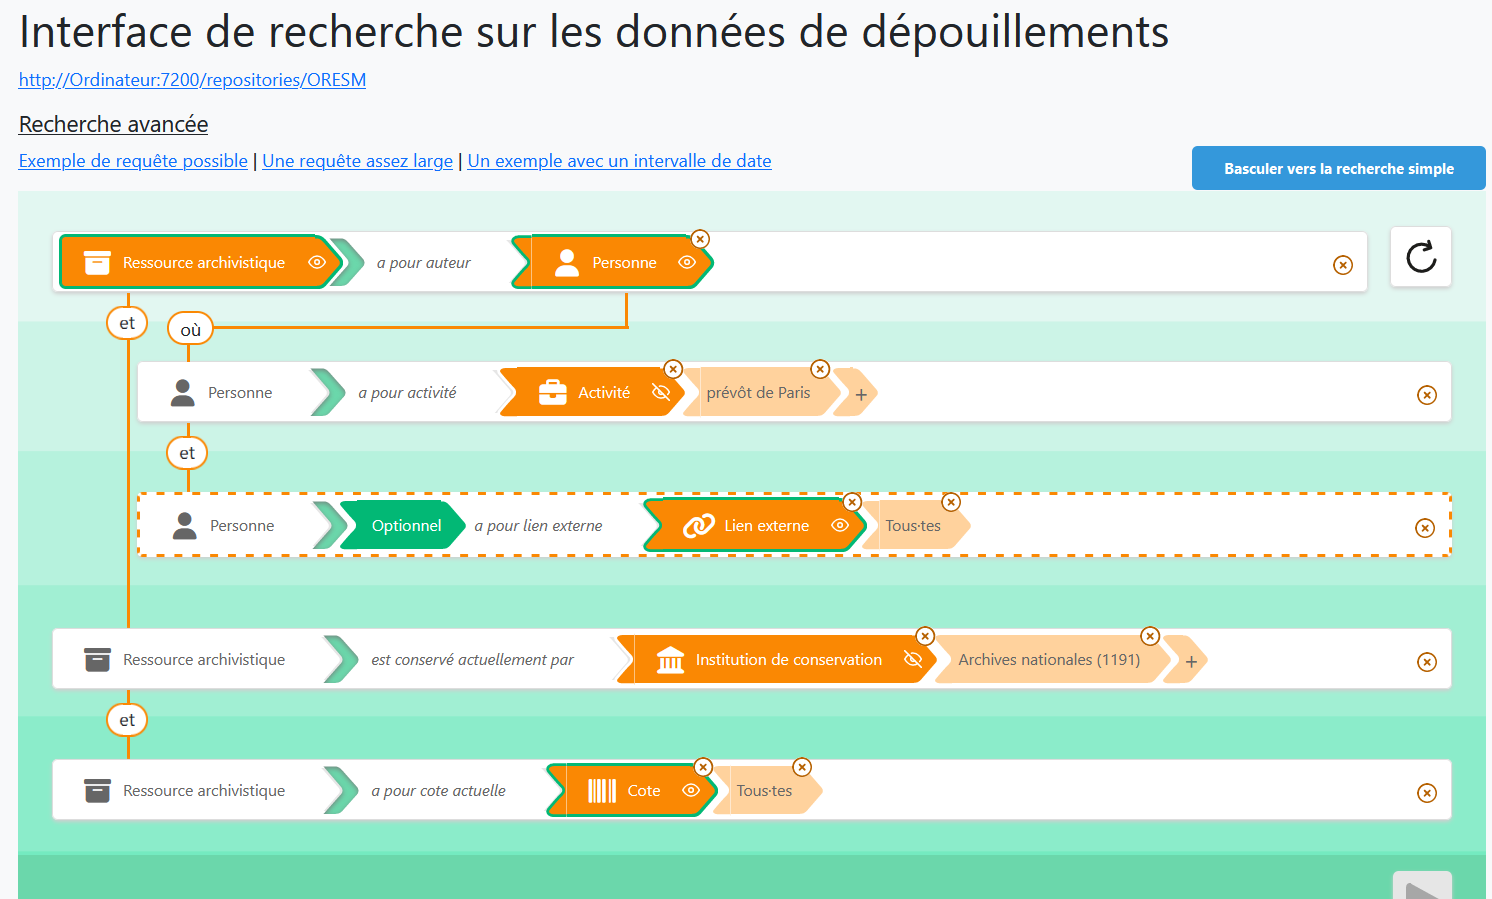
\includegraphics[width=1\linewidth]{images/interface-oresm-exemple.png}
    \caption{Exemple d'une requête avancée conçue à partir de l'interface Sparnatural.}
    \label{fig:recherche-avancée}
    \centering
    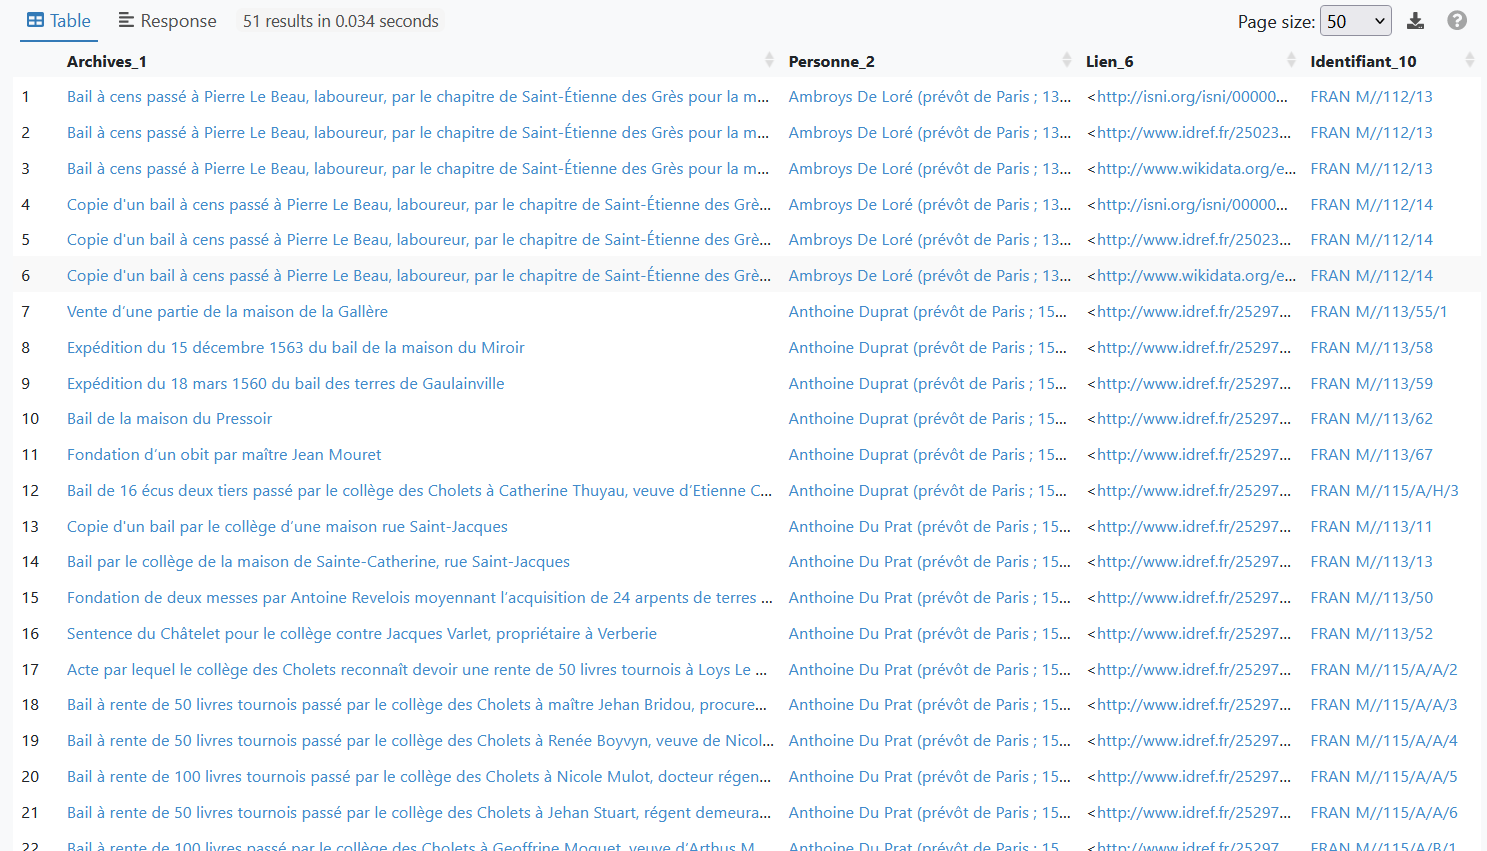
\includegraphics[width=1\linewidth]{images/resultat-requete-sparnatural.png}
    \caption{Le résultat de la requête. Les labels de chaque éléments sont affichés, ce sont des liens vers l'URI de l'entité.}
    \label{fig:resultat-sparnatural}
\end{figure}

\par
Il faut toutefois remettre les choses dans le contexte de notre stage, pour lequel nous ne disposions que d'un temps très limité. Cette interface a été avant tout réalisée pour prendre l'outil en main. Avec celui-ci nous avons testé notre modèle de données. Grâce à Sparnatural nous pouvons illustrer les possibilités offertes avant de lancer un recueil de besoins. Nous avions besoin d'un support suffisamment complet et développé à remettre aux chercheurs. Avec cette configuration temporaire ils auront une base pour faire des commentaires, émettre des envies et indiquer ce qui ne va pas. La base de donnée et l'interface ont été déployées par Sébastien Clément sur un serveur test de la BIS pour préparer cette étape. Il nous faut avoir en tête que notre travail devra répondre avant tout aux besoins des futurs utilisateurs du portail ORESM. L'ensemble de cette interface ne sera pas le résultat mis en ligne mais plutôt le moyen de faire éprouver l'ensemble de la preuve de concept réalisée dans le cadre de ce stage aux différents acteurs du projet.